\documentclass{../../../oss-ap12ibhl}

\usepackage[siunitx]{circuitikz}
\tikzset{voltage dir=RP}

\begin{document}
\genheader

\gentitle{13}{DC CIRCUIT ANALYSIS}
\begin{questions}
  \question Which of the following statements best summarizes a series circuit
  with three different resistances?
  \begin{choices}
    \choice In all parts of the circuit, the resistances are different, the
    voltage drops are the same, and the current is different.
    \choice In all parts of the circuit, the resistances are the same, the
    voltage drops are the same, and the current is different.
    \choice In all parts of the circuit, the resistances are different, the
    voltage drops are different, and the current is the same.
    \choice In all parts of the circuit, the resistances are different, the
    voltage drops are the same, and the current is the same.
    \choice In all parts of the circuit, the resistances are the same, the
    voltage drops are the same, and the current is the same.
  \end{choices}
  \vspace{.7in}

  \uplevel{
    \textbf{Questions \ref{series1}--\ref{series4}}
    \begin{center}
      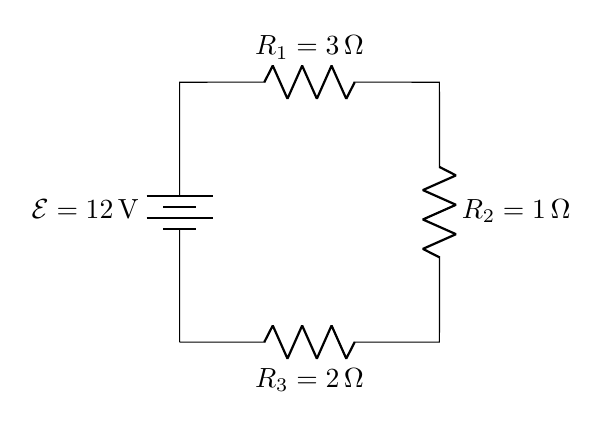
\begin{tikzpicture}[american voltages,scale=1.1]
        \draw(0,0)
        to[battery,l=\mbox{$\mathcal{E}=\SI{12.}{\volt}$}] (0,3)
        to[R=\mbox{$R_1=\SI{3.}{\ohm}$}] (3,3)
        to[R=\mbox{$R_2=\SI{1.}{\ohm}$}] (3,0)
        to[R=\mbox{$R_3=\SI{2.}{\ohm}$}] (0,0);
      \end{tikzpicture}
    \end{center}
  }
  
  \question What is the current flowing through the circuit shown in the
  diagram?
  \begin{choices}
    \choice\SI{1}{\ampere}
    \choice\SI{2}{\ampere}
    \choice\SI{4}{\ampere}
    \choice\SI{6}{\ampere}
    \choice\SI{12}{\ampere}
  \end{choices}
  \label{series1}
    
  \question Which of the following statements is true about the circuit shown
  in the diagram?
  \begin{choices}
    \choice The voltage drop is greatest across $R_1$, but $R_1$ has the least
    amount of current flowing through it.
    \choice The voltage drop is greatest across $R_2$, but $R_2$ has the least
    amount of current flowing through it.
    \choice The voltage drop is greatest across $R_3$, but $R_3$ has the least
    amount of current flowing through it.
    \choice The voltage drops and current are equal across all resistors.
    \choice The voltage drop is greatest across $R_1$, but the current is
    equal at all points in the circuit.
  \end{choices}
  \vspace{.7in}
    
  \question In this diagram, what is the power dissipated by all of the
  resistors in the circuit?
  \begin{choices}
    \choice\SI{2}{W}
    \choice\SI{6}{W}
    \choice\SI{12}{W}
    \choice\SI{24}{W}
    \choice\SI{48}{W}
  \end{choices}
  
  \question In the diagram, what is the voltage drop across the third resistor
  ($R_3$)?
  \begin{choices}
    \choice\SI{2}{V}
    \choice\SI{3}{V}
    \choice\SI{4}{V}
    \choice\SI{6}{V}
    \choice\SI{12}{V}
  \end{choices}
  \label{series4}
    
  \question Two identical resistors with resistance $R$ are connected in
  series with a power supply with a potential difference of $\Delta V$. Which
  expression represents the power output of the entire circuit?
  \begin{choices}
    \choice $\dfrac{\Delta V^2}{4R}$
    \choice $\dfrac{\Delta V^2}{2R}$
    \choice $\dfrac{\Delta V^2}{R}$
    \choice $\dfrac{2(\Delta V)^2}{R}$
    \choice $2R(\Delta V)^2$
  \end{choices}

  \question Two identical resistors with resistance $R$ are connected in
  parallel with a power supply with a potential difference of $\Delta V$.
  Which expression represents the rate that the circuit transfers energy to a
  single resistor?
  \begin{choices}
    \choice $\dfrac{\Delta V^2}{4R}$
    \choice $\dfrac{\Delta V^2}{2R}$
    \choice $\dfrac{\Delta V^2}{R}$
    \choice $\dfrac{2(\Delta V)^2}{R}$
    \choice $2R(\Delta V)^2$
  \end{choices}

  \uplevel{
    \textbf{Questions \ref{parallel1}--\ref{parallel4}}
    \begin{center}
      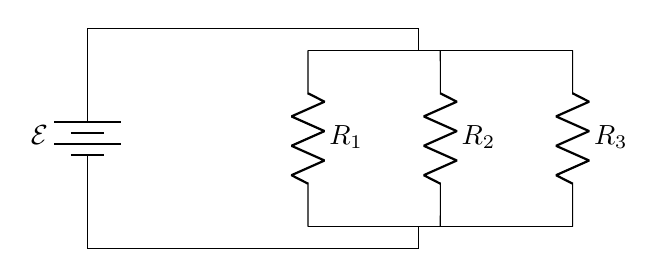
\begin{tikzpicture}[american voltages,scale=1.4]
        \draw(0,0) to[battery,l=$\mathcal{E}$] (0,2)--(3,2)--(3,1.8);
        \draw(2,1.8)--(4.4,1.8);
        \draw(2,0.2)--(4.4,0.2);
        \draw(2,1.8) to[R=$R_1$] (2,0.2);
        \draw(3.2,1.8) to[R=$R_2$] (3.2,0.2);
        \draw(4.4,1.8) to[R=$R_3$] (4.4,0.2);
        \draw(3,0.2)--(3,0)--(0,0);
      \end{tikzpicture}
      
      \vspace{.1in}$\mathcal{E}=\SI{12.}{V}$, $R_1=\SI{10.}{\ohm}$,\\
      $R_2=\SI{6.}{\ohm}$, $R_3=\SI{8.}{\ohm}$
    \end{center}
  }
    
  \question For the circuit in the diagram, which of the following
  expressions will describe the amount of current flowing through the
  resistors?
  \label{parallel1}
  \begin{choices}
    \choice $I_1=I_2=I_3$
    \choice $I_3>I_2>I_1$
    \choice $I_1>I_2<I_3$
    \choice $I_2>I_1>I_3$
    \choice $I_1<I_2<I_3$
  \end{choices}
    
  \question For the circuit in the diagram, what is the equivalent resistance?
  \begin{choices}
    \choice\SI{0.040}{\ohm}
    \choice\SI{0.40}{\ohm}
    \choice\SI{1.0}{\ohm}
    \choice\SI{2.6}{\ohm}
    \choice\SI{24}{\ohm}
  \end{choices}
    
  \question For the circuit in the diagram, what is the total current?
  \begin{choices}
    \choice\SI{0.5}{\ampere}
    \choice\SI{4.6}{\ampere}
    \choice\SI{12}{\ampere}
    \choice\SI{30}{\ampere}
    \choice\SI{300}{\ampere}
  \end{choices}
    
  \question For the circuit in the diagram, the third resistor ($R_3$)
  dissipates how much energy each second?
  \label{parallel4}
  \begin{choices}
    \choice\SI{12}{\watt}
    \choice\SI{14}{\watt}
    \choice\SI{46}{\watt}
    \choice\SI{212}{\watt}
    \choice\SI{300}{\watt}
  \end{choices}
    
%  \item Two resistors made of the same material are shown in the figure. A
%    current of $I$ flows through the left resistor when connected to a
%    potential difference of $V$. What current will flow through the right
%    resistor when connected to the same potential?
%
%    \vspace{-.2in}
%    \begin{center}
%      \pic{.45}{resistors.png}
%    \end{center}
%    \begin{enumerate}[noitemsep,topsep=0pt,leftmargin=18pt,label=(\Alph*)]
%    \item $I/2$
%    \item $I/4$
%    \item $I$
%    \item $2I$
%    \item $4I$
%    \end{enumerate}
%  \end{enumerate}

  \uplevel{
    \textbf{Questions \ref{3resistors1}--\ref{3resistors2}}
    \cpic{.45}{r-in-series}
  }
  \question Which is the correct ranking of the currents for the resistors?
  \label{3resistors1}
  \begin{choices}
    \choice $I_A = I_B = I_C$
    \choice $I_A > I_B > I_C$
    \choice $I_C > I_A = I_B$
    \choice $I_C > I_B > I_A$
    \choice $I_C < I_B < I_A$
  \end{choices}

  \question Which is the correct ranking of the potential differences of the
  resistors?
  \label{3resistors2}
  \begin{choices}
    \choice $V_A = V_B = V_C$
    \choice $V_A > V_B > V_C$
    \choice $V_A = V_B > V_C$
    \choice $V_C > V_B > V_A$
    \choice $V_C < V_B < V_A$
  \end{choices}
  \newpage
  
  \uplevel{
    \textbf{Questions \ref{cap1}--\ref{cap2}}
    \begin{center}
      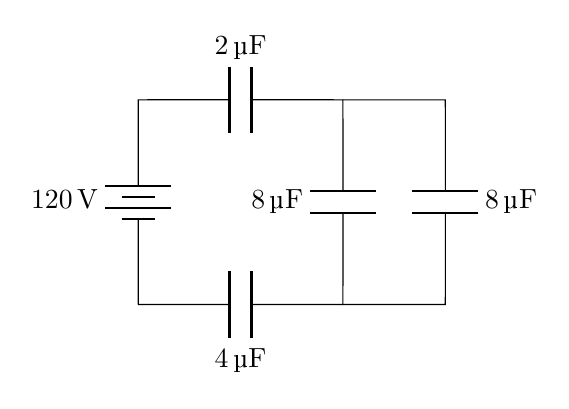
\begin{tikzpicture}[american voltages,scale=1.3]
        \draw(0,0) to[battery,l=\mbox{\SI{120}{\volt}}] (0,2)
        to[C,l=\mbox{\SI2{\micro\farad}}](2,2)
        to[C,l_=\mbox{\SI8{\micro\farad}}](2,0)
        to[C,l=\mbox{\SI4{\micro\farad}}](0,0);
        \draw(2,2)--(3,2) to[C=\mbox{\SI8{\micro\farad}}] (3,0)--(2,0);
      \end{tikzpicture}
    \end{center}
  }
  
  \question The equivalent capacitance of this circuit is
  \begin{choices}
    \choice\SI{7/4}{\micro\farad}
    \choice\SI{4/7}{\micro\farad}
    \choice\SI{21/16}{\micro\farad}
    \choice\SI{10}{\micro\farad}
    \choice\SI{22}{\micro\farad}
  \end{choices}
  \label{cap1}
    
  \question The charge stored on the \SI{2}{\micro\farad} capacitor is most
  nearly
  \begin{choices}
    \choice \SI{6}{\micro\coulomb}
    \choice \SI{12}{\micro\coulomb}
    \choice \SI{22}{\micro\coulomb}
    \choice \SI{36}{\micro\coulomb}
    \choice \SI{120}{\micro\coulomb}
  \end{choices}
  \label{cap2}
  
  \question A capacitor $C_0$ is connected to a battery and stores charge. If
  the space between the capacitor plates is filled with oil, which of the
  following quantities increase?
  \begin{choices}
    \choice Capacitance and voltage across the plates
    \choice Charge and voltage across the plates
    \choice Capacitance and electric field between the plates
    \choice Capacitance and charge on the plates
    \choice Electric field between the plates and voltage across the plates
  \end{choices}

%  \textbf{Question 16--17}
%  
%  The circuit shows a capacitor, a battery, and a resistor. Switch $S$ is first
%  connected to point $a$ to charge the capacitor, then a long time later
%  switched to point $b$ to discharge the capacitor through the resistor.
%  \begin{center}
%    \begin{tikzpicture}[american voltages,scale=1.5]
%      \draw(0,0) to[battery=$\mathcal{E}$](0,2) to[short,-*] (1.5,2);
%      %node[pos=1,above]{a};
%      \draw(2.5,2) to[short,*-] (3.5,2) to[R=$R$,] (3.5,0)--(0,0);
%      \draw(2,0) to[C=$C$,-*] (2,1.25);
%      \draw(2,1.25)--(2.3,2.15) node[pos=1,above]{s};
%      \node at (1.5,1.8) (a){a};
%      \node at (2.5,1.8) (b){b};
%    \end{tikzpicture}
%  \end{center}
%  
%  \item The maximum current through the resistor is
%    \begin{enumerate}[noitemsep,topsep=0pt,leftmargin=18pt,label=(\Alph*)]
%    \item $\mathcal{E}/2R$
%    \item $\mathcal{E}/R$
%    \item $\mathcal{E}/RC$
%    \item $\mathcal{E}/2RC$
%    \item $C\mathcal{E}/R$
%    \end{enumerate}
%  \end{enumerate}
%  \columnbreak
%  \textbf{Questions 18--20}
%  \begin{enumerate}[leftmargin=18pt,resume]
%  \item The spherical capacitor shown consists of a conducting shell of radius a
%    inside a larger conducting shell of radius b. A charge $−Q$ is placed on the
%    inner sphere and a charge $+Q$ is placed on the outer shell. The
%    capacitance of the capacitor is $C_0$. The magnitude of the electric field
%    $E$ at a distance $r$ between the spheres is
%    \begin{center}
%      \begin{tikzpicture}[scale=.65]
%        \draw(0,0) circle(1);
%        \draw(0,0) circle(3);
%        \fill(0,0) circle(.1);
%        \draw[->](0,0)--(1,0) node[midway,above]{a};
%        \draw[->,rotate=-140](0,0)--(3,0) node[midway,left]{b};
%        \begin{scope}[rotate=160]
%          \draw[->](0,0)--(2,0) node[midway,above]{r};
%          \fill(2,0) circle(.1);
%        \end{scope}
%        \node at (0,3.3) (a){$+Q$};
%        \node at (0,1.3) (b){$-Q$};
%      \end{tikzpicture}
%    \end{center}
%    \begin{enumerate}[noitemsep,topsep=0pt,leftmargin=18pt,label=(\Alph*)]    
%    \item $\displaystyle\frac{Q}{4\pi\epsilon_0r^2}$
%    \item $\displaystyle\frac{Q}{4\pi\epsilon_0r}$
%    \item $\displaystyle\frac{Q}{4\pi\epsilon_0a^2}$
%    \item $\displaystyle\frac{Q}{4\pi\epsilon_0b^2}$
%    \item zero
%    \end{enumerate}
%
%  \item The bottom half of the space between the spheres is filled with oil of
%    dielectric constant $\kappa=3$, creating two capacitors connected to each
%    other. Which of the following is true of the two capacitors?
%    \begin{center}
%      \begin{tikzpicture}[scale=.65]
%        \draw[fill=gray!60](-1,0)--(-3,0) arc(180:360:3)--(1,0) arc(0:-180:1);
%        \draw(0,0) circle(1);
%        \draw(0,0) circle(3);
%        \fill(0,0) circle(.1);
%        \draw[->,rotate=230](0,0)--(1,0) node[midway,above left]{a};
%        \draw[->](0,0)--(3,0) node[pos=0.7,above]{b};
%        \node at (0,3.3) (a){$+Q$};
%        \node at (0,1.3) (b){$-Q$};
%      \end{tikzpicture}
%    \end{center}
%    \begin{enumerate}[noitemsep,topsep=0pt,leftmargin=18pt,label=(\Alph*)]
%    \item They are connected in series.
%    \item They are connected in parallel.
%    \item The total capacitance has not changed.
%    \item The total capacitance of the spheres has decreased.
%    \item The total capacitance is now zero.
%    \end{enumerate}
%    \columnbreak

  \question A battery of voltage $V_0$ is attached to two parallel conducting
  plates. Charge is distributed on the plates, and then the battery is
  removed. A dielectric is then inserted between the plates, filling the
  space. Which of the following decreases after the battery is removed and the
  dielectric is inserted to fill the space between the plates?
  \begin{choices}
    \choice Capacitance
    \choice Charge on the plates
    \choice Net electric field between the plates
    \choice Area of the plates
    \choice Separation distance between the plates
  \end{choices}
    
  \question Circuit I and Circuit II shown each consist of a capacitor and a
  resistor. A battery is connected across a and b, and then removed. Which of
  the following statements is true of the circuits?
  \begin{center}
    Circuit I\\
    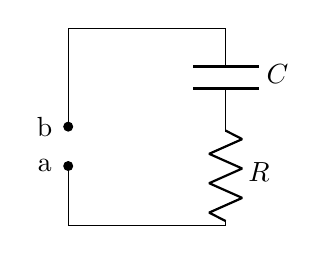
\begin{tikzpicture}
      \draw(0,1.25) to[short,*-](0,2.5)--(2,2.5) to[C=$C$](2,1.25)
      to[R=$R$](2,0)--(0,0) to[short,-*](0,0.75);
      \node at (-0.3,0.75) {a};
      \node at (-0.3,1.25) {b};
    \end{tikzpicture}
    
    Circuit II\\
    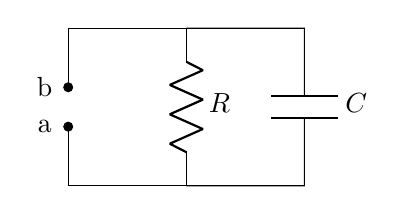
\begin{tikzpicture}
      \draw(0,1.25) to[short,*-](0,2)--(1.5,2) to[R=$R$](1.5,0)--(0,0)
      to[short,-*](0,0.75);
      \draw(1.5,2)--(3,2) to[C=$C$](3,0)--(1.5,0);
      \node at (-0.3,0.75) {a};
      \node at (-0.3,1.25) {b};
    \end{tikzpicture}
  \end{center}
  \begin{choices}
    \choice Circuit I and Circuit II will both retain stored energy when the
    battery is removed.
    \choice Neither Circuit I nor Circuit II will retain stored energy when
    the battery is removed.
    \choice Only Circuit I will retain stored energy when the battery is
    removed.
    \choice Only Circuit II will retain stored energy when the battery is
    removed.
    \choice Current will continue to flow in both circuits after the battery
    is removed.
  \end{choices}

  \uplevel{
    \centering
    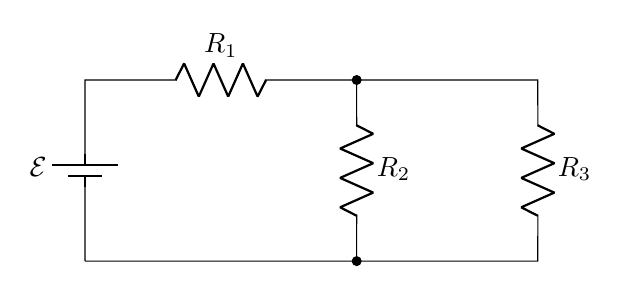
\begin{tikzpicture}[american voltages,scale=2.3]
      \draw(0,0) to[battery1,l=$\mathcal{E}$](0,1) to[R,l=$R_1$,-*](1.5,1)
      to[R,l=$R_2$,-*](1.5,0)--(0,0);
      \draw(1.5,1)--(2.5,1) to[R,l=$R_3$](2.5,0)--(1.5,0);
    \end{tikzpicture}
  }
  \question A simple circuit consisting of three resisotrs is shown above.
  $R_1$ had the same resistance as $R_2$, and $R_2$ has twice the resistance
  of $R_3$. Determine the ratio of the heat dissipated of $R_1$ to $R_2$.
  \begin{choices}
    \choice $1:9$
    \choice $1:3$
    \choice $1:1$
    \choice $3:1$
    \correctchoice $9:1$
  \end{choices}

% TAKEN FROM THE 2016 AP PHYSICS 1 EXAM FREE-RESPONSE QUESTION #4
  \uplevel{
    \cpic{.3}{dc1}
  }
  \question A circuit contains a battery and four identical resistors arranged
  as shown in the diagram above.
  \begin{parts}
    \part Rank the magnitude of the potential difference across each resistor
    from greatest to least. If any resistors have potential differences with
    the same magnitude, state that explicitly. Briefly explain your reasoning.

    \vspace{.1in}Ranking:
    
    \vspace{.3in}Brief explanation:
    
    \uplevel{
      \vspace{.3in}Resistor $B$ is now removed from the circuit, and there is no
      connection between the wires that were attached to it. The new circuit
      diagram is shown below.
      \begin{center}
        \pic{.3}{dc2}
      \end{center}
    }

    \part When resistor $B$ is removed, does the current through resistor $A$
    increase, decrease, or remain the same? Explain your reasoning.

    \vspace{.1in}
    \underline{\hspace{.3in}} Increase\hspace{.2in}
    \underline{\hspace{.3in}} Decrease\hspace{.2in}
    \underline{\hspace{.3in}} Remain the same
   
    
    \part When resistor $B$ is removed, does the current through resistor $C$
    increase, decrease, or remain the same? Briefly explain your reasoning.

    \vspace{.1in}
    \underline{\hspace{.3in}} Increase\hspace{.2in}
    \underline{\hspace{.3in}} Decrease\hspace{.2in}
    \underline{\hspace{.3in}} Remain the same
  \end{parts}
  \newpage

%\item The figure shows a circuit with two resistors, a battery, a capacitor,
%  and a switch. Originally, the switch is open, and the capacitor is
%  uncharged.
%  \begin{center}
%    \begin{tikzpicture}[scale=1.4,american voltages]
%      \draw[thick] (2,0)
%      to[battery1,l=\mbox{\SI{12}{\volt}},*-*] (0,0)
%      to[short,-*] (0,1.5)
%      to[R,l=\mbox{$R_1=\SI{15}{\ohm}$},-*] (2,1.5)--(2,0);
%
%      \draw[thick](0,1.5)
%      to[short,-*] (0,3)
%      to[C,l=\mbox{\SI{240}{\micro\farad}}] (1,3)
%      to[R=\mbox{$R_2=\SI{10}{\ohm}$},-*] (2,3)--(2,1.5);
%    \end{tikzpicture}
%  \end{center}
%  \begin{enumerate}
%  \item Complete the voltage-current-resistance-power (VIRP) chart for
%    the circuit immediately after the switch is closed.
%    \bgroup
%    \def\arraystretch{1.8}
%    
%    {\large
%      \begin{center}
%        \begin{tabular}{l|m{1.2cm}|m{1.2cm}|m{1.2cm}|m{1.2cm}}
%          \hline
%          \textbf{Location} & \textbf{\emph{V}} & \textbf{\emph{I}} &
%          \textbf{\emph{R}} & \textbf{\emph{P}}\\ \hline
%          1 & & & \SI{15}{\ohm} & \\ \hline
%          2 & & & \SI{10}{\ohm} & \\ \hline
%          Total for Circuit & \SI{12}{\volt}& & & \\\hline
%        \end{tabular}
%      \end{center}
%    }
%    \egroup
%  \item Complete the voltage-current-resistance-power (VIRP) chart for
%    the circuit after the switch is closed for a long time.
%        \bgroup
%    \def\arraystretch{1.8}
%    
%    {\large
%      \begin{center}
%        \begin{tabular}{l|m{1.2cm}|m{1.2cm}|m{1.2cm}|m{1.2cm}}
%          \hline
%          \textbf{Location} & \textbf{\emph{V}} & \textbf{\emph{I}} &
%          \textbf{\emph{R}} & \textbf{\emph{P}}\\ \hline
%          1 & & & \SI{15}{\ohm} & \\ \hline
%          2 & & & \SI{10}{\ohm} & \\ \hline
%          Total for Circuit & \SI{12}{\volt}& & & \\\hline
%        \end{tabular}
%      \end{center}
%    }
%    \egroup
%  \item What is the energy stored in the capacitor after the switch has
%    been closed a long time?
%  \end{enumerate}
%  \newpage

  %TAKEN FROM 2003 AP PHYSICS B FREE-RESPONSE QUESTION #2
  \uplevel{
    \begin{center}
      \pic{.3}{rc-circuit}
    \end{center}
  }
  \question A circuit contains two resistors (\SI{10}{\ohm} and \SI{20}{\ohm})
  and two capacitors (\SI{12}{\micro\farad} and \SI6{\micro\farad}) connected to
  a \SI6{\volt} battery, as shown in the diagram above. The circuit has been
  connected for a long time.
  \begin{parts}
    \part Calculate the total capacitance of the circuit.
    \part Calculate the current in the \SI{10}{\ohm} resistor.
    \part Calculate the potential difference between points $A$ and $B$.
    \part Calculate the charge stored on one plate of the \SI6{\micro\farad}
    capacitor.
    \part The wire is cut at point $P$. Will the potential difference between
    points $A$ and $B$ increase, decrease, or remain the same? Justify your
    answer.

    \vspace{.1in}
    \underline{\hspace{.5in}} increase\hspace{.3in}
    \underline{\hspace{.5in}} decrease\hspace{.3in}
    \underline{\hspace{.5in}} remain the same
  \end{parts}
  \newpage

  %TAKEN FROM 2015 AP PHYSICS 2 EXAM FREE-RESPONSE QUESTION #2
  \uplevel{
    \cpic{.45}{bulbs}
  }
  \question A battery of emf $\mathcal{E}$ and negligible internal resistance,
  three identical incandescent lightbulbs, and a switch $S$ that is initially
  open are connected in the circuit shown above. The bulbs each have resistance
  $R$. Students make predictions about what happens to the brightness of the
  bulbs after the switch is closed.
  \begin{parts}
    \part A student makes the following prediction about bulb 1: ``Bulb 1 will
    decrease in brightness when the switch is closed.''
    \begin{subparts}
      \subpart Do you agree or disagree with the student's prediction about
      bulb 1? Qualitatively explain your reasoning.
      
      \subpart Before the switch is closed, the power expended by bulb 1 is
      $P_1$. Derive an expression for the power $P_\text{new}$ expended by bulb 1
      after the switch is closed in terms of $P_1$.
      %\vspace{1.5in}
      
      \subpart How does the result of your derivation in part (a)ii relate to
      your explanation in part (a)i?
      %\vspace{1in}
    \end{subparts}
    \part A student makes the following prediction about bulb 2: ``Bulb 2 will
    decrease in brightness after the switch is closed.''
    \begin{subparts}
      \subpart Do you agree or disagree with the student's prediction about bulb
      2? Explain your reasoning in words.
      %\vspace{1.5in}
      
      \subpart Justify your explanation with a calculation.
      %\vspace{1.5in}
    \end{subparts}
    
    \part While the switch is open, bulb 3 is replaced with an uncharged
    capacitor. The switch is then closed.
    \begin{subparts}
      \subpart How does the brightness of bulb 1 compare to the brightness of
      bulb 2 immediately after the switch is closed? Justify your answer.
      %\vspace{1.5in}
      \subpart How does the brightness of bulb 1 compare to the brightness of
      bulb 2 a long time after the switch is closed? Justify your answer.
    \end{subparts}
  \end{parts}
  \newpage

  % TAKEN FROM 2012 AP PHYSICS B EXAM FREE-RESPONSE QUESTION #5
  \uplevel{
    \cpic{.4}{bulbs2}
  }
  \question Four lightbulbs are connected in a circuit with a \SI{24}{\volt}
  battery as shown above.
  \begin{parts}
    \part
    \begin{subparts}
      \subpart Determine the average potential energy change of an electron as
      it moves from point $Z$ to point $X$.
      \subpart Indicate whether the electron gains or loses potential energy as
      it moves from point $Z$ to point $X$.

      \vspace{.1in}
      \underline{\hspace{.5in}} Gains energy\vspace{.3in}
      \underline{\hspace{.5in}} Loses energy
    \end{subparts}
    \part Calculate the equivalent resistance of the circuit.
    \part
    \begin{subparts}
      \subpart Calculate the magnitude of the current through point $Y$.
      \subpart Indicate on the diagram the direction of the current through
      point $Y$.
    \end{subparts}
    \part Calculate the energy dissipated in the \SI{12}{\watt} bulb in 5 s.
    \part Rank the bulbs in order of brightness, with 1 being the brightest. If
    any bulbs have the same brightness, give them the same ranking.

    \vspace{.1in}
    \underline{\hspace{.5in}} Bulb A\hspace{.3in}
    \underline{\hspace{.5in}} Bulb B\hspace{.3in}
    \underline{\hspace{.5in}} Bulb C\hspace{.3in}
    \underline{\hspace{.5in}} Bulb D
  \end{parts}
  \newpage

  % TAKEN FROM 2002 AP PHYSICS B EXAM FREE-RESPONSE QUESTION #3
  \question Two lightbulbs, one rated \SI{30}{\watt} at \SI{120}{\volt} and
  another rated \SI{40}{\watt} at \SI{120}{\volt}, are arranged in two
  different circuits.
  \begin{parts}
    \part The two bulbs are first connected in parallel to a \SI{120}{\volt}
    source.
    \begin{subparts}
      \subpart Determine the resistance of the bulb rated \SI{30}{\watt} and
      the current in it when it is connected in this circuit.
      
      \subpart Determine the resistance of the bulb rated 40 W and the current
      in it when it is connected in this circuit.
    \end{subparts}

    \part The bulbs are now connected in series with each other and a
    \SI{120}{\volt} source.
    \begin{subparts}
      \subpart Determine the resistance of the bulb rated \SI{30}{\watt} and
      the current in it when it is connected in this circuit.
      
      \subpart Determine the resistance of the bulb rated \SI{40}{\watt} and
      the current in it when it is connected in this circuit.
      \end{subparts}

    \part In the spaces below, number the bulbs in each situation described, in
    order of their brightness. (1 = brightest, 4 = dimmest)

    \vspace{.1in}
    \underline{\hspace{.4in}} \SI{30}{\watt} bulb in the parallel circuit
    
    \underline{\hspace{.4in}} \SI{40}{\watt} bulb in the parallel circuit

    \underline{\hspace{.4in}} \SI{30}{\watt} bulb in the series circuit

    \underline{\hspace{.4in}} \SI{40}{\watt} bulb in the series circuit
    \vspace{.1in}

    \part Calculate the total power dissipated by the two bulbs in each of
    the following cases.

    \begin{subparts}
      \subpart The parallel circuit
      \subpart The series circuit
    \end{subparts}
  \end{parts}
\end{questions}
\end{document}
